\documentclass[a4paper,12pt,twoside]{article}

\usepackage[utf8]{inputenc}
\usepackage[T2A]{fontenc}
\usepackage[english]{babel}
\usepackage{booktabs}
\usepackage[margin = 1in,includeheadfoot]{geometry}
\usepackage{graphicx}
\usepackage{amsmath}
\usepackage{amssymb}
\usepackage{tikz}
\usepackage{fancyhdr}

\parindent=0pt
\parskip=10pt

\pagestyle{fancy}
\fancyhf{}
\rhead{Sasha Petrov}
\lhead{}
\rfoot{\thepage}
\setlength{\headheight}{14.5pt}

%hyperlinks package -- should be the last to import
\usepackage{hyperref}
\hypersetup{
	colorlinks = true,
	linkcolor=blue,
	citecolor=blue,
	urlcolor=blue }
	
\title{ECON 31703: Assignment 2}
\author{Sasha Petrov}

\usepackage{Sweave}
\begin{document}
\Sconcordance{concordance:ps2.tex:ps2.Rnw:%
1 34 1 1 0 6 1 1 6 3 1 1 3 1 0 1 2 9 0 1 3 6 1 1 3 12 0 1 3 12 1 1 4 2 %
0 1 1 1 3 2 0 1 1 6 0 1 4 16 1 1 4 7 0 1 3 3 1 1 3 19 0 1 3 5 1 1 4 7 0 %
2 3 19 0 1 3 10 1}


\maketitle

\section*{Exercise 1}



\subsection*{(d), (e)}

\begin{Schunk}
\begin{Sinput}
> zero <- sapply(blasso, function(x) {TRUE %in% (x[[1]] != 0)})
> print(paste('how many times do we get non-zero coefs?', sum(zero)))
\end{Sinput}
\begin{Soutput}
[1] "how many times do we get non-zero coefs? 0"
\end{Soutput}
\begin{Sinput}
> 
\end{Sinput}
\end{Schunk}


Not sure what is the point in applying lasso with $\lambda = 20$ to a DGP with unit variance. Looks like the approximate maximum value $\sum_{i = 1}^N y_i^k x_{ik}$ can take is around $N$, which makes it very unlikely for the coefficient estimate to exceed $20$. At least in the simulations, I didn't get any non-zero coefs.

\textit{How to read the table:} Rows -- two coefficient estimates ($\hat \beta_1$ and $\hat \beta_2$); 1st column -- OLS, 2nd column -- lasso with $\lambda = 20$,
3rd column -- ridge with $\lambda = 20$.

\begin{Schunk}
\begin{Sinput}
> print(comp)
\end{Sinput}
\begin{Soutput}
          [,1] [,2]       [,3]
[1,]  1.001317    0  0.6657135
[2,] -1.000447    0 -0.6665185
\end{Soutput}
\begin{Sinput}
> 
\end{Sinput}
\end{Schunk}

The pattern of coefficients conforms with what we expect OLS, lasso, and ridge to do.
Thanks to the independence between most regressors, OLS does a good job of estimating the true values. Rdige only does shrinking, so we just see the reduction of coefs towards $0$. Lastly, lasso does both shrinking and thresholding; and because we chose such a high $\lambda$, we end up doing only thresholding.


\subsection*{f}

Given the chosen algorithm to find the lasso estimate (coordinate-wise decent), the sufficient condition for all coefficient estimates to be $0$ is (it's definitely sufficient, not sure about necessity; if this condition is not met, then at least in the first step there'll be a `meaningful' updating; does it mean that it's not possible that this updated coefficient will be pushed back to $0$? I don't know):

\begin{equation}
	\left|\frac{1}{N} \sum_{i = 1}^N y_i^k x_{ik} \right| < \lambda, \, \forall k = 1, \dots, p \quad \textrm{and} \quad y_i^k = y_i - \sum_{j \neq k} x_{ij}  \hat\beta_j^0
\end{equation}

\begin{Schunk}
\begin{Sinput}
> plot(0, 0, xlim = c(0, 1), ylim = c(-1, 1), type = 'n',
+      xlab = expression(lambda), ylab = expression(hat(beta)))
> cl <- rainbow(5)
> for (i in 1:5) {
+   lines(grid, coefs_1f[i, ], col = cl[i])
+ }
> legend("topright", legend = 1:5, col=cl, pch=1)
> 
> 
\end{Sinput}
\end{Schunk}
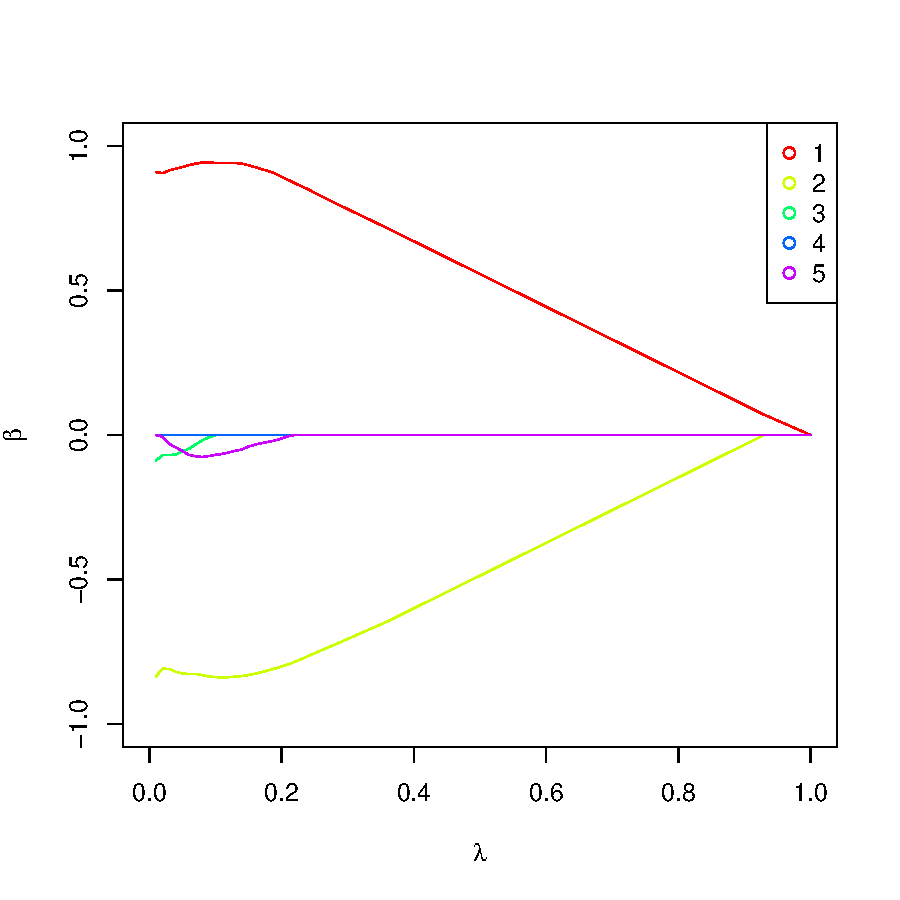
\includegraphics{ps2-004}

The figure clearly shows how lasso behaves: as penalisation becomes stricter, lasso shrinks more and more (might be even to $0$).


\textit{The whole standardisation issue:} To be honest, still don't quite understand a) why it's especially important with lasso compared to ols (for which the scale also obviously matters); b) how should one compare results for ols and lasso -- standardise for both or rescale lasso coefs `back'? In the given case it doesn't seem to matter; that is, lasso (with standardised data) gives estimates of the magnitude comparable to ols run on non-standardised data. Is this purely because the data is generated from the standard normal CDF?


\section*{Exercise 2}

$\rho = 0.9$ means that once $X_0$ gets realised, all other $\{X_t\}_{t = 1}^{200}$ will be `approximately' the same; which implies that it's hard to estimate $\beta$ (I expect variance of the estimate to be high, as the variance of draws from $X_t$ is very low).

\textit{Another observations about forecasting:} At the same time, this is also the only reason forecasting possible, right? We're not really interested in estimating $Y_t$ as a function of $X_t$, because once $X_t$ is realised, so is $Y_t$. So, the `path dependence' of $X_t$ is what gives us hope that we can predict $Y_{t + h}$ with $X_t$. In other words, the crux of the issue here is not that we don't know what effect of some treatment is (we don't care about changing $X_t$); we actually care only about the level of the `regression function' but we don't know what the actual `treatment' is.

All this makes me wonder: why do we pose the problem in such a `reduced-form' way? That is, finding the predictor of $Y_{t + h}$ given $X_t$. Can we gain anything by a) estimating $Y_t$ as a function of $X_t$ (which has a better `feel' in terms of reflecting the actual reality); b) then predicting $X_{t + h}$ with $X_t$? Is there a result that predicting directly $Y_{t + h}$ from $X_t$ has no `deficiencies' compared to what I just proposed?

\subsection*{(b)}

\begin{Schunk}
\begin{Sinput}
> plot(lambdas, av_mspe, ylim = c(7.8, 12),
+      xlab = expression(lambda), ylab = expression(bar(MSPE)))
> 
\end{Sinput}
\end{Schunk}
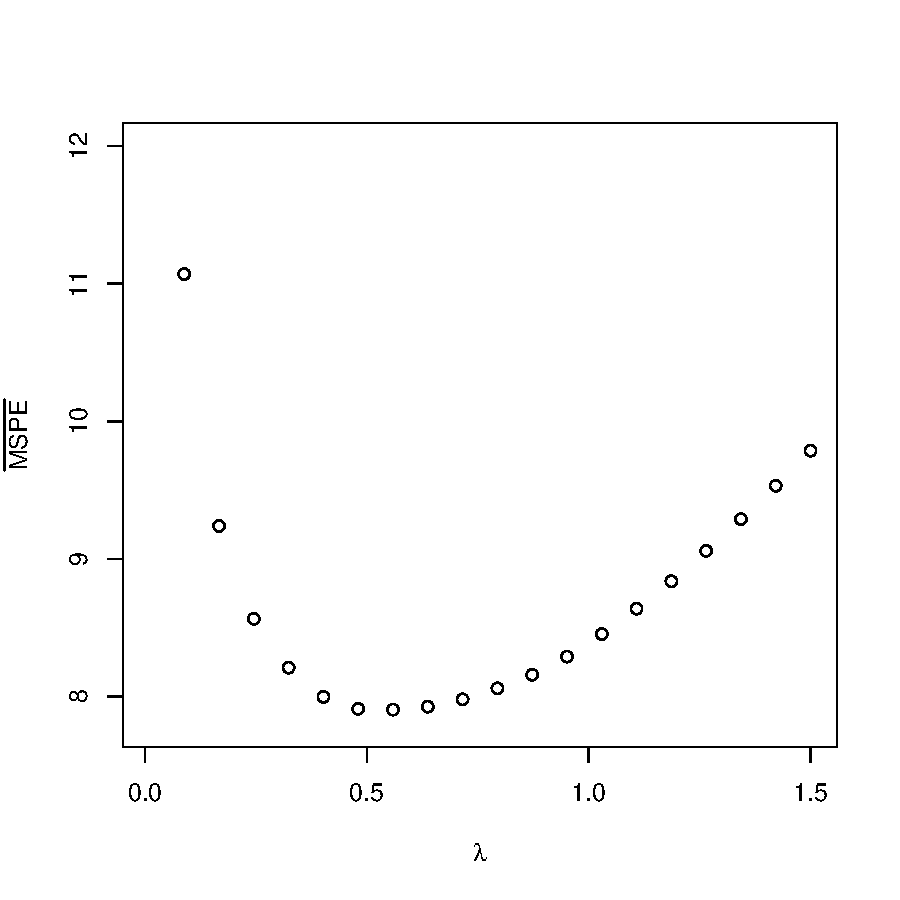
\includegraphics{ps2-005}

I think I got a typical cross-validation plot: a U-shaped average MSPE graph; no penalisation (low $\lambda$) makes multicollinearity concerns dominate; too much penalisation (high $\lambda$) leads to a very high bias. But there is a sweet spot.


\begin{Schunk}
\begin{Sinput}
> table_2b
\end{Sinput}
\begin{Soutput}
 [1]  3.417707e+00  0.000000e+00 -6.944767e-03  0.000000e+00 -7.103123e-03
 [6]  0.000000e+00  4.503338e-03  0.000000e+00  0.000000e+00  0.000000e+00
[11] -2.246265e-03 -1.949425e-02  0.000000e+00  0.000000e+00 -4.668151e-03
[16]  0.000000e+00  0.000000e+00  0.000000e+00  0.000000e+00 -3.608411e-03
[21]  0.000000e+00  0.000000e+00 -1.424678e-03  0.000000e+00  0.000000e+00
[26]  0.000000e+00 -1.973268e-03  7.466889e-05  0.000000e+00 -9.091331e-03
[31]  0.000000e+00  3.177821e-03  0.000000e+00  0.000000e+00  0.000000e+00
[36]  0.000000e+00  0.000000e+00  0.000000e+00  4.363195e-03  0.000000e+00
[41]  0.000000e+00  0.000000e+00  0.000000e+00  0.000000e+00  0.000000e+00
[46] -1.841665e-03  0.000000e+00  0.000000e+00 -1.626328e-02  0.000000e+00
\end{Soutput}
\begin{Sinput}
> 
\end{Sinput}
\end{Schunk}

The estimate of $\beta_1$ using the `best' $\lambda$ ($\approx 3.4$) is considerably away from the true model (although not clear if that's a valid comparison -- $\beta_1 = 5$ is for the contemporaneous model, right?). If you want to think about it this way, then probably could make an observation that although the coefficient is very much away from truth, the prediction of the output is pretty good.


\subsection*{(c)}

\begin{Schunk}
\begin{Sinput}
> plot(lambdas, av_mspe_c, ylim = c(7.8, 11),
+      xlab = expression(lambda), ylab = expression(bar(MSPE)))
> 
\end{Sinput}
\end{Schunk}
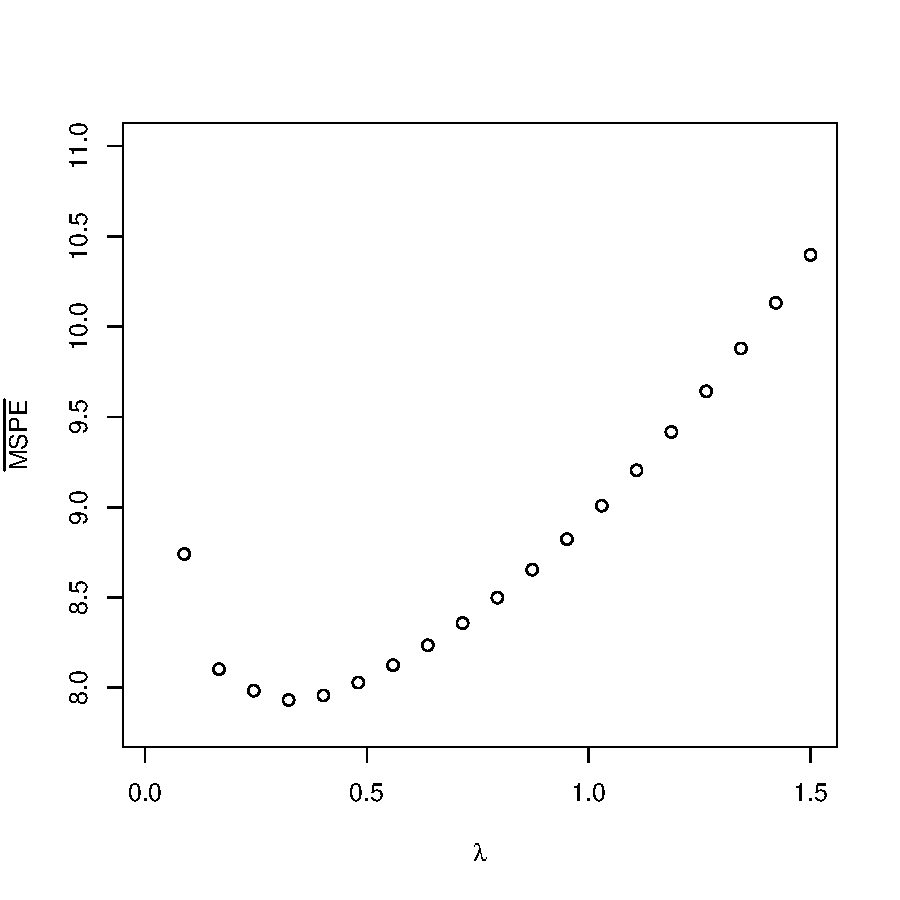
\includegraphics{ps2-007}

\begin{Schunk}
\begin{Sinput}
> table_2c
\end{Sinput}
\begin{Soutput}
 [1]  3.774599e+00  2.180659e-03  2.369225e-02  1.087551e-01  2.215690e-02
 [6]  5.155484e-02  3.708250e-03  1.458426e-02  1.544257e-02  2.535052e-02
[11]  0.000000e+00  0.000000e+00  0.000000e+00 -3.119166e-03  0.000000e+00
[16] -4.250995e-03  7.924166e-04  0.000000e+00  0.000000e+00  9.632805e-03
[21] -7.307604e-03  1.139970e-02 -1.450787e-03  0.000000e+00 -9.683384e-04
[26]  2.533053e-03  0.000000e+00 -2.252555e-03 -1.563290e-02  4.205165e-03
[31]  0.000000e+00 -1.081249e-03  0.000000e+00  0.000000e+00 -1.014561e-02
[36] -4.594677e-05 -1.090371e-03 -5.779976e-04  0.000000e+00  3.272237e-03
[41]  0.000000e+00  0.000000e+00  1.115021e-02  6.604177e-04 -4.752210e-03
[46]  0.000000e+00 -7.887697e-03  7.814161e-03  0.000000e+00  9.182347e-03
\end{Soutput}
\begin{Sinput}
> 
\end{Sinput}
\end{Schunk}


Some observations when there's correlation between regressors:

\begin{itemize}
  \item Computation time increased significantly. I guess, coordinate-wise decent has to make more `loops' chasing spurious correlations.
  \item There are more non-zero coefficients in the end result. Probably for the same reason as above.
  \item The cross-validated optimal $\lambda$ is lower in the correlation case. Maybe because with higher penalisastion we risk penalising the actually important coefficients because of the `spurious' correlation among regressors?
\end{itemize}

\end{document}
